
\section*{\centering \large Lembar Pengesahan Program Studi Teknik Informatika}

\addcontentsline{toc}{section}{Lembar Pengesahan}  % Manually add to ToC
\setcounter{page}{2}

\begin{center}
\vspace{1cm}

\Large  % Increase font size for the main title
\textbf{Analisis Rekapitulasi Data Pemilih Tetap Pilkada 2024 Provinsi Lampung Menggunakan K-Means Clustering}

\vspace{1cm}
\Large
di KPU Provinsi Lampung

\vspace{2cm}

\large  % Switch back to large for the author's name
Oleh: \\
Arsyadana Estu Aziz  \\
121140068

\vspace{2cm}

\large  % Same size for this text for consistency
disetujui dan disahkan sebagai \\
Laporan Praktek Kerja Lapangan

\end{center}

\vfill

\noindent \normalsize  % Apply the large size explicitly for the bottom section
Lampung Selatan, 15 November 2024 \\
Pembimbing Praktek Kerja Lapangan Program Studi Teknik Informatika ITERA

% \noindent Meida Cahyo Untoro, S.Kom., M.Kom \\
% NIP: 19890518 201903 1 011
\begin{figure}[b]
    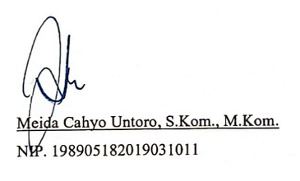
\includegraphics[width=0.5\linewidth]{images/signature_meida.jpg}
    \label{fig:enter-label}
\end{figure}

\begin{center}
\large
\textbf{Lembar Pengesahan Program Studi Teknik Informatika}

\vspace{1cm}

\Large
\textbf{Analisis Rekapitulasi Data Pemilih Tetap Pilkada 2024 Provinsi Lampung Menggunakan K-Means Clustering}

\vspace{1cm}
\Large
di KPU Provinsi Lampung

\vspace{2cm}

Oleh: \\
Arsyadana Estu Aziz  \\
121140068

\vspace{2cm}

disetujui dan disahkan sebagai \\
Laporan Praktek Kerja Lapangan


\end{center}
\vfill

% \noindent Bandar Lampung, 5 Agustus 2024 \\
% Kassubag Data dan Informasi KPU Provinsi Lampung

% \vspace{3cm}

% \noindent Ressy Silvia Dewi, S.E., M.M. \\
% NIP: 198306092009022005
\begin{figure}[b]
    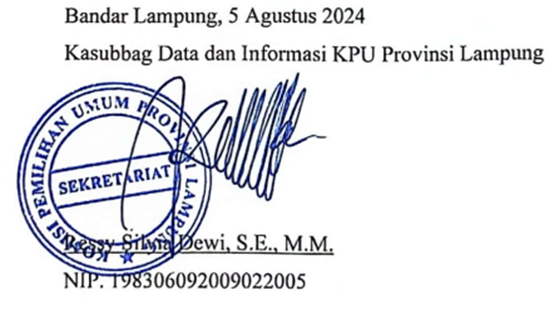
\includegraphics[width=0.5\linewidth]{images/signature_ressy.png}
    \label{fig:enter-label}
\end{figure}

\newpage